% !TEX encoding = UTF-8 Unicode

% Beispiel für ein LaTeX-Dokument im Format "seminarvorlage"
\documentclass[ngerman]{seminarvorlage}
% ngerman = Deutsch in neuer Rechtschreibung, alternativ english
\usepackage{babel}[german] % automatische Sprachunterstützung

\usepackage[utf8]{inputenc} % Kodierung der Non-ASCII-Zeichen
\usepackage[T1]{fontenc} % Moderne Fonts, Trennung von Wörtern mit Umlauten
\usepackage{cleveref} % für bequeme Referenzen, siehe \cref unten

\usepackage{embrac}% upright brackets in emphasised text, () and [], empfohlen

%\usepackage{biblatex}% besser als bibtex, aber dann biber statt bibtex benutzen
\begin{document}

% Unbedingt angeben: Titel, Autoren
% Freiwillig: Adresse, E-Mail
\title{Vergleich binärer und nicht-binärer Serialisierungsformate}
\numberofauthors{2}
\author{
  \alignauthor Matthias Raba \\
    \email{i22029@hb.dhbw-stuttgart.de}
  \alignauthor Fabian Noll\\
    \email{i22024@hb.dhbw-stuttgart.de}
}

\maketitle% Titelangaben produzieren, aber kein Inhaltsverzeichnis, \tableofcontents funktioniert nicht!


\abstract{In dieser Arbeit werden binäre und nicht-binäre Serialisierungsformate verglichen mit dem Ziel, ihre Eignung für diverse Anwendungsbereiche zu evaluieren. Im Fokus stehen die Formate JSON, XML, ProtoBuf und MessagePack, die hinsichtlich ihrer Geschwindigkeit, Speicherbedarf und Wartbarkeit/Nutzbarkeit untersuchet werden. Durch eine Reihe von Tests und Analysen wird die Leistung der Formate in verschiedenen Szenarien bewertet und  deren Stärken und Schwächen beleuchtet. Darüber hinaus werden die  jeweiligen Vor- und Nachteile in spezifischen Anwendungsgebieten erörtert, um eine Entscheidungsgrundlage für die Auswahl eines passenden Serialisierungsformats in der Praxis zu bieten.}

\keywords{Serialisierung, JSON, XML, ProtoBuf, 
MessagePack, Binär, Nicht-binäre,
Datenformatvergleich, Anwendungsgebiete}

% Section-Überschriften werden automatisch in GROSSBUCHSTABEN gesetzt
\section{Einleitung}
Die Serialisierung von Daten ist eine wesentliche Technik in der modernen Softwareentwicklung, die den Austausch und die Persistenz von Informationen zwischen Systemen ermöglicht. In der heutigen Vielfalt an Serialisierungsformaten stehen Entwickler vor der Herausforderung, das richtige Format für spezifische Anwendungsfälle zu wählen. Dabei spielen Aspekte wie Effizienz, Lesbarkeit, Wartbarkeit und Kompatibilität eine entscheidende Rolle. Diese Arbeit untersucht und vergleicht ausgewählte binäre und nicht-binäre Serialisierungsformate – JSON, XML, Protocol Buffers und MessagePack – unter Berücksichtigung objektiver Kriterien wie Geschwindigkeit, Speicherbedarf und Implementierungsgüte. Ziel ist es, eine systematische Bewertung der Formate zu liefern, die als Orientierungshilfe für praktische Entscheidungen dient. Der Beitrag dieser Analyse liegt nicht nur in der Gegenüberstellung der technischen Merkmale, sondern auch in der Berücksichtigung von Anwendungsbereichen und realen Herausforderungen bei der Implementierung.

% Jede Section am besten mit einem Kommentar hier im Quelltext markieren
\section{Grundlagen}

Das folgende Kapitel beschäftigt sich mit grundlegenden Begriffen, die für das Verständnis der weiteren Ausführungen unabdinglich sind.

% Kurze Definition von Serialisierung und Deserialisierung
\subsection{Serialisierung und Deserialisierung}
Serialisierung bezeichnet den Prozess der Umwandlung komplexer Datenstrukturen oder Objekte in ein lineares Datenformat, das für die Speicherung oder Übertragung in verschiedenen Medien geeignet ist, wie beispielsweise Dateien oder Netzwerkprotokolle. Deserialisierung hingegen beschreibt den Vorgang, bei dem das lineare Datenformat analysiert und in die ursprüngliche Datenstruktur zurückgeführt wird. Diese Prozesse sind essenziell für die Persistenz von Daten und die Kommunikation zwischen verteilten Systemen.

\subsection{Binäre vs. Nicht-Binäre Formate}
Binäre und nichtbinäre Serialisierungsformate unterscheiden sich grundlegend in der Art und Weise, wie sie Daten speichern und übertragen. Binäre Formate wie Protobuf oder MessagePack codieren Daten in einem kompakten, maschinenlesbaren Format, was ihnen eine hohe Effizienz sowohl hinsichtlich der Speichernutzung als auch der Verarbeitungsgeschwindigkeit verleiht. Diese Formate sind ideal für Systeme, in denen Performance eine zentrale Rolle spielt, wie bei der Kommunikation zwischen Microservices oder in Anwendungen mit begrenzter Bandbreite. Ein Nachteil dieser Formate ist jedoch, dass sie nicht von Menschen direkt gelesen werden können. Dies bedeutet, dass spezielle Tools oder Software nötig sind, um den Inhalt zu interpretieren, was die Fehlersuche und das Debuggen erschweren kann.

Nichtbinäre Formate wie XML oder JSON speichern Daten in einem textbasierten, menschenlesbaren Format. Ein klarer Vorteil ist die einfache Lesbarkeit und Bearbeitbarkeit, da Entwickler und Nutzer ohne spezielle Software die Inhalte direkt inspizieren und ändern können. Diese Eigenschaft macht sie besonders geeignet für Konfigurationsdateien, Datenformate, die von Menschen überprüft werden müssen, oder APIs, bei denen Klarheit und Transparenz im Vordergrund stehen. Der Nachteil liegt in der ineffizienteren Speichernutzung und der geringeren Performanz, da diese Formate mehr Speicherplatz benötigen und der Parsing-Prozess langsamer ist als bei binären Formaten. XML zum Beispiel erzeugt durch seine umfangreichen Tags oft eine größere Datenmenge, während JSON kompakter ist, aber dennoch die Nachteile von Textformaten teilt.

In Bezug auf den Einsatzbereich sind binäre Formate aufgrund ihrer Effizienz und hohen Geschwindigkeit in Bereichen wie Embedded Systems, Kommunikationsprotokollen und Cloud-basierten Diensten weit verbreitet. Nichtbinäre Formate hingegen finden häufig in Bereichen Anwendung, in denen eine einfache Handhabung und schnelle Lesbarkeit durch Menschen wichtiger sind als die absolute Performance, wie z.B. bei Datenübertragungen im Web oder bei einfachen Konfigurationsdateien. Während binäre Formate eine bessere Performance und Speicheroptimierung bieten, sind textbasierte Formate flexibler und einfacher in der Nutzung und im Austausch.
 
\subsection{Serialisierung vs. Komprimierung}

Serialisierung muss grundsätzlich von Komprimierung unterschieden werden. In der Praxis werden oft beide Methoden verwendet, um die zu speichernde Datenmenge zu minimieren. Serialisierung bezeichnet jede wohldefinierte Strukturierung von Daten. Diese erfolgt beispielsweise zum Zweck der Persistierung oder um Daten zuverlässig zwischen Rechnersystemen zu transportieren, zum Beispiel über Netzwerkverbindungen hinweg. Komprimierung hingegen bezeichnet die allgemeine Verringerung der Datengröße. Komprimierung kann entweder verlustfrei oder verlustbehaftet stattfinden. Somit sind die beiden Verfahren fundamental verschieden, können allerdings in Kombination verwendet werden. So können in einem Serialisierungsformat bereits komprimierte Daten gespeichert werden, oder es wird die zuerst serialisierte Datenmenge anschließend komprimiert. Damit die Betrachtungen und Vergleiche zwischen den Messergebnissen in den folgenden Kapiteln aussagekräftig sind, wird auf Komprimierung verzichtet. Allgemein kann ein beliebiger Komprimierungsalgorithmus verwendet werden, um die Speichereffizienz zu erhöhen. Die nachfolgenden Betrachtungen sollen aber die Serialisierungsformate an sich bewerten.

\subsection{Theoretisch optimale Serialisierung}

Jedes Serialisierungsformat hat ein unteres Limit bezüglich des benötigten Speicherplatzes eines serialisierten Datensatzes. Für diese Betrachtung werden folgende Datentypen angenommen: 

\begin{table}[h]
  \centering
  \begin{tabular}{|l|l|l|} 
  \hline
  Datentyp  & Wertebereich               & Arbeitsspeicher                    \\ 
  \hline
  i32         & $-\left(2^{31}-1\right)$ bis $2^{31}$  & 32 Bits              \\
  f32         & $\pm 10^{38}$              & 32 Bits                          \\
  boolean     & {[}true, false]            & 8 Bits                           \\
  $string_n$  & $[0, 1114112]^n$           & $8 \cdot n \leq 32 \cdot n$ Bits \\
  \hline
  \end{tabular}
  \caption{Wertebereich und Speicherverbraucher gängiger primitiver Datentypen}
\end{table}

Die aufgeführten Größen sind in vielen gängigen Programmiersprachen vertreten (C, C++, Java, Rust). Bei Zeichenketten wird von einer UTF-8 kompatiblen Implementation ausgegangen. Moderne Programmiersprachen unterstützen die effizientere Darstellung von mehreren Booleans in einem Byte. Da dies aber nicht in jeder Sprache der Fall ist, wird diese Optimierung nicht berücksichtigt.

Unabhängig vom Serialisierungsformat muss verarbeitende Software wissen, welche Struktur die Daten haben. Diese Struktur kann entweder durch die Syntax des Serialisierungsformats vorgegeben oder durch andere Mechanismen definiert werden. JSON und Protobuf sind jeweils Beispiele für beide Mechanismen. Da JSON ein text-basiertes, nichtbinäres Format ist, ist die Typzugehörigkeit aus dem serialisierten Datum ersichtlich. Die Definition der Syntax von JSON garantiert, dass die Wertebereiche der Datentypen sich nicht überschneiden. Protobuf hat diese Metainformation grundsätzlich nicht, da es auf ``rohen'' binären Datensätzen arbeitet. Die Grenzen sowie die Datentypen der einzelnen Serialisierten Feldern können nicht aus dem Datensatz gewonnen werden. Daher benötigt Protobuf eine externe Datei, die die Struktur der Datensätze beschreibt. Da diese \texttt{.proto} Dateien vergleichsweise klein sind (wenige kB), werden sie bei dieser Betrachtung vernachlässigt. Wird keine solche externe Strukturdefinition verwendet, ist es notwendig, durch festgelegte Zeichenketten, auch ``Delimiter'' genannt, die Grenzen der Datenfelder kennzuzeichnen.

\subsubsection{Binäre Formate}

In binären Formaten werden die primitiven Datentypen effizient abgebildet, da die serialisierte bereits der deserialisierten Form entspricht. Angenommen, die Struktur wird durch eine externe Definition gegeben, entsteht kein Overhead im Vergleich zur nativen Repräsentation im Arbeitsspeicher. Allerdings kann es notwendig sein, die Endianness bei der Serialisierung zu verändern, was keinen Einfluss auf die Größe des Datums hat.

\subsubsection{Nichtbinäre Formate}

Bei nichtbinären Formaten muss eine Transformation zwischen der binären und der textuellen Form der Daten vorgenommen werden. Für diese Transformation gilt:

$$ M_{\text{textuell}} \geq M_{\text{binär}} $$

Angenommen, das Serialisierungsziel unterstützt UTF-8, benötigen Strings keine solche Transformation, da sie direkt übernommen werden können. Viele Serialisierungsformate benötigen allerdings Delimiter, um den Anfang und das Ende des Strings anzuzeigen. Zusätzlich kann es notwendig sein, im Format als Steuerzeichen verwendete Zeichen zu modifizieren, damit sie von den Steuerzeichen unterscheidbar bleiben. Viele Formate verwenden dazu z.B. das Präfix `\textbackslash\textbackslash' oder `/'.

Die minimale Größe eines einzelnen Zeichens sind 8 Bits. Daraus folgt, dass auch Booleans mindestens mit einem Zeichen repräsentiert werden. Daher gilt auch für Booleans $ M_{\text{textuell}} \geq M_{\text{binär}} $. Viele Formate verwenden die Literale ``true'' und ``false'', um die Lesbarkeit zu erhöhen. Angenommen, beide Werte treten gleich häufig auf, wird die Effizienz damit um den Faktor $\frac{4 + 5}{2} = 4.5$ gesenkt.

Für die Serialisierung von Integern wird ebenfalls von einer Gleichverteilung im Wertebereich angenommen. Dies ist in reellen Anwendungen nicht zwingend der Fall, beispielsweise sind kleinere Zahlen weitaus häufiger vertreten \cite{berger2015introduction}. Für die weitere Betrachtung wird dennoch die Gleichverteilung angenommen, da sie eine breite und theoretisch durchschnittliche Einschätzung ermöglicht. Zur Berechnung der durchschnittlichen Länge eines solchen Integers muss zunächst die durchschnittliche Anzahl der Dezimalstellen erfasst werden. Die Anzahl der Ganzzahlen mit n Stellen ist durch $10^n$ gegeben. Allerdings werden hierbei führende Nullen nicht berücksichtigt. Folgende Tabelle zeigt die tatsächliche Verteilung der positiven Ganzzahlen:

\begin{table}[H]
  \centering
  \begin{tabular}{|l|l|l|l|} 
  \hline
  \textbf{Untere Grenze} & \textbf{Obere Grenze} & \textbf{Anzahl} & \textbf{Ziffern}         \\ 
  \hline
  0                      & 9                     & 10              & 1                        \\
  10                     & 99                    & 90              & 2                        \\
  100                    & 999                   & 900             & 3                        \\
  1000                   & 9999                  & 9000            & 4                        \\
  10000                  & 99999                 & 90000           & 5                        \\
  100000                 & 999999                & 900000          & 6                        \\
  1000000                & 9999999               & 9000000         & 7                        \\
  10000000               & 99999999              & 90000000        & 8                        \\
  100000000              & 999999999             & 900000000       & 9                        \\
  1000000000             & 2147483648            & 1147483649      & 10                       \\
  \hline
  \end{tabular}
  \caption{Verteilung positiver Ganzzahlen 32-Bit Integer}
\end{table}

Das arithmetische Mittel der Länge wird wie folgt berechnet:

$$\frac{\sum_{i=1}^{10} Anzahl(i) * Dezimalstellen(i)}{2^{31}} \approx 9.4826$$

Da die Zahlen von 0-9 in UTF-8 mit nur einem Zeichen und damit nur einem Byte repräsentiert werden, sind die durchschnittliche Anzahl an Dezimalstellen und der durchschnittliche Speicherverbrauch der gleichen Zahl identisch. Allerdings führt die Tabelle nur die positiven Zahlen auf. Negative Zahlen werden üblicherweise über das vorangestellte Symbol `-' deklariert. Da der Zahlenraum der positiven und negativen Zahlen nahezu gleich groß sind, ergibt sich daraus eine durchschnittliche Erhöhung der Länge um 0.5 Zeichen. Somit ist die durchschnittliche Länge eines textuell serialisierten 32-Bit Integers 9.9826 Byte. Da ein nativer Integer in nur 4 Bytes repräsentiert wird, ist die textuelle Repräsentation im Durchschnitt um 149.56\% größer. Somit gilt auch für Integer $ M_{\text{textuell}} \geq M_{\text{binär}} $.

Ähnliche Berechnungen sind auch für Fließkommazahlen möglich, allerdings ist die Repräsentation, im Gegensatz zu den Ganzzahlen, implementationsabhängig. Dabei gibt es verschiedene Merkmale, die festlegen, ab wann die wissenschaftliche Notation verwendet wird. Allerdings lässt bereits der enorme abbildbare Zahlenraum von $\pm10^{38}$ darauf schließen, dass die benötigte Anzahl an Dezimalstellen die der Ganzzahlen weit übersteigt. Zusätzliche Zeichen und Zeichenketten, wie etwa der Dezimalpunkt oder der Exponent in der wissenschaftlichen Notation erhöhen die Anzahl der benötigten Zeichen zusätzlich.

\section{Kriterien}

Zum Vergleich von Serialisierungsverfahren ist die Auswahl geeigneter Metriken entscheidend, um fundierte und vergleichbare Ergebnisse zu erzielen. Die folgenden Metriken wurden festgesetzt und mit Fachliteratur abgeglichen und bieten eine umfassende Grundlage für den Vergleich:

\textbf{Serialisierungszeit}\newline
Diese Metrik misst die Zeit, die benötigt wird, um Datenstrukturen in ein spezifisches Format zu konvertieren. Eine geringere Serialisierungszeit kann die Effizienz von Anwendungen erhöhen, insbesondere in zeitkritischen Systemen. Die Messung erfolgt durch Zeitstempel vor und nach dem Serialisierungsprozess, wobei die Differenz die benötigte Zeit ergibt.

\textbf{Deserialisierungszeit}\newline
Sie erfasst die Dauer, die erforderlich ist, um serialisierte Daten zurück in ihre ursprüngliche Struktur zu überführen. Eine schnelle Deserialisierung ist essenziell für Anwendungen, die zügig auf gespeicherte oder übertragene Daten zugreifen müssen. Die Messmethodik entspricht derjenigen der Serialisierungszeit, mit Fokus auf den Deserialisierungsprozess.

\textbf{Kompressionsrate}\newline
Sie gibt das Verhältnis der Größe der originalen Daten zur Größe der serialisierten Daten an. Eine höhere Kompressionsrate reduziert den Speicherbedarf und die Bandbreitennutzung, was besonders in ressourcenbeschränkten Umgebungen von Vorteil ist. Die Berechnung erfolgt durch Division der Größe der ursprünglichen Daten durch die Größe der serialisierten Daten.

\textbf{Implementierungsgüte}\newline
Die Implementierungsgüte betrachtet, wie die Performance der Serialisierungsverfahren in unterschiedlichen Programmiersprachen variiert. Diese Messung erfolgt durch den Vergleich der ermittelten Metriken über verschiedene Implementierungen hinweg. Dabei zeigt sich, dass die Implementierungsgüte ein entscheidender Faktor ist, der nicht vernachlässigt werden darf. Wie bereits in \textit{Object serialization analysis and comparison in java and .net} \cite{10.1145/944579.944589} gezeigt, kann die gleiche Technologie in zwei vermeintlich ähnlichen Sprachumgebungen wie Java und .NET erhebliche Leistungsunterschiede aufweisen. In der dort beschriebenen Analyse performte XML in .NET je nach Objekttyp und Datengröße zwischen 65 \% und 85 \% besser als in Java. Dies verdeutlicht, wie wichtig es ist, nicht nur das Serialisierungsformat selbst, sondern auch dessen spezifische Implementierung in der Zielumgebung zu berücksichtigen.

\textbf{Nutzbarkeit/Wartbarkeit}\newline
Diese qualitative Metrik bewertet, wie einfach ein Serialisierungsverfahren zu implementieren, zu nutzen und zu warten ist. Aspekte wie Dokumentation, Community-Unterstützung und die Komplexität der Integration spielen hierbei eine Rolle. Die Bewertung erfolgt durch Experteneinschätzungen und Benutzerfeedback.

\textbf{Ressourcenverbrauch}\newline
Diese Metrik misst die Nutzung von Systemressourcen wie CPU, Speicher und, falls relevant, auch Energie während der Serialisierungs- und Deserialisierungsprozesse. Ein effizienter Ressourcenverbrauch ist entscheidend, insbesondere in Umgebungen mit begrenzten Systemressourcen, wie eingebetteten Systemen oder IoT-Geräten. Diese Metrik wird einfacher bewertet in Bezug auf Probleme oder limitationen die sich während der Testreihen kristallisiert haben.

Metriken wie Serialisierungszeit, Deserialisierungszeit und Kompressionsrate gehören zu den zentralen Kriterien eines Vergleichs von Serialisierungsverfahren. . Diese Aspekte werden in nahezu jeder relevanten Publikation als entscheidend hervorgehoben, darunter insbesondere die Arbeiten von Hericko et al. \cite{10.1145/944579.944589} sowie Maeda \cite{6215346}. Ebenso spielt die Implementierungsgüte eine bedeutende Rolle, wie beispielsweise in den Werken von Hericko et al. \cite{10.1145/944579.944589} und Vanura und Kriz \cite{vanura2018perfomance} aufgezeigt wird. Dort wird verdeutlicht, dass die Wahl der Programmiersprache – etwa Java oder \text{C\#/.NET} – Performanceunterschiede von bis zu einem Faktor 2 verursachen kann. Auch die Nutzbarkeit und Wartbarkeit stellen wichtige Metriken dar, die sowohl von den Autoren dieser Arbeit als auch von den beteiligten Stakeholdern als relevant angesehen werden.

\section{Die Serialisierungsformate}

Im folgenden Abschnitt wird die Auswahl der zu vergleichenden Formate erläutert als auch die ausgewählten Formate in einer kurzen Zusammenfassung vorgestellt.

\subsection{Begründung der Formatwahl}

Die Auswahl der Formate JSON, XML, Protocol Buffers und MessagePack erfolgte aufgrund ihrer unterschiedlichen Stärken, die jeweils auf spezifische Anwendungsfälle und Anforderungen abzielen.

\textbf{JSON} \cite{rfc8259} wurde wegen seiner Einfachheit, Lesbarkeit und breiten Unterstützung in Web-Technologien gewählt. Es ist ideal für Situationen, in denen menschliche Lesbarkeit und einfache Integration in verschiedene Programmiersprachen wichtig sind. Es ist weit verbreitet und wird beispielsweise oft in Webanwendungen zur Kommunikation mit Serverschnittstellen verwendet. Auch für einfache Loggingzwecke wird das Format oft verwendet.

\textbf{XML} \cite{w3c_xml} wurde aufgrund seiner Flexibilität und umfassenden Unterstützung für strukturierte Daten gewählt. Es ist besonders geeignet für Anwendungen, die eine strenge Validierung und Unterstützung für umfangreiche Metadaten erfordern, wie in vielen Legacy-Systemen oder dokumentenzentrierten Umgebungen.

\textbf{Protocol Buffers} \cite{protobuf} wurden aufgrund ihrer hohen Effizienz und der Fähigkeit, komplexe Datenstrukturen zu serialisieren, ausgewählt. Sie sind ideal für leistungsorientierte Anwendungen, in denen Geschwindigkeit und geringer Speicherbedarf entscheidend sind, wie bei der Kommunikation zwischen Microservices oder in mobilen Anwendungen.

\textbf{MessagePack} \cite{msgpack} ergänzt die Auswahl durch seine Effizienz in der Datenspeicherung und -übertragung, was es zu einer ausgezeichneten Wahl für ressourcenbeschränkte Umgebungen macht. Diese Diversität an Formaten ermöglicht es, verschiedene Szenarien optimal abzudecken, von einfacher Web-Kommunikation bis hin zu hochperformanten, ressourcenoptimierten Anwendungen.

\subsection{Vorstellung der Formate}

\textbf{JSON (JavaScript Object Notation)} \cite{rfc8259}
JSON ist ein textbasiertes Serialisierungsformat, das durch seine Einfachheit und Struktur überzeugt. Es speichert Daten in Form von Schlüssel-Wert-Paaren, Arrays und verschachtelten Objekten, die leicht von Maschinen verarbeitet und von Menschen gelesen werden können. JSON hat sich besonders in der Webentwicklung etabliert, da es direkt von JavaScript unterstützt wird, was die Interoperabilität zwischen Frontend und Backend erleichtert. Viele Web-APIs nutzen JSON, um Daten zwischen Client und Server auszutauschen. Die breite Unterstützung in verschiedenen Programmiersprachen macht JSON zu einem universellen Standard für viele Anwendungsfälle. JSON ist nicht auf Webanwendungen beschränkt, sondern findet auch in Konfigurationsdateien, Datenbanken wie MongoDB und bei der Interprozesskommunikation Anwendung. Allerdings hat JSON auch Einschränkungen, darunter ein höherer Speicherbedarf und eine geringere Verarbeitungsgeschwindigkeit im Vergleich zu binären Formaten. Ein weiteres potenzielles Problem ist das Fehlen einer strikten Typisierung, was in größeren Projekten zu Fehleranfälligkeit führen kann. Dennoch bleibt JSON aufgrund seiner Balance zwischen Lesbarkeit und Funktionalität ein unverzichtbares Werkzeug in der modernen Softwareentwicklung.

\textbf{MessagePack} \cite{msgpack}
MessagePack ist ein binäres Serialisierungsformat, das entwickelt wurde, um die Effizienz von Datenübertragungen zu maximieren. Im Gegensatz zu textbasierten Formaten wie JSON oder XML speichert MessagePack Daten in einem kompakten binären Format, was die Dateigröße erheblich reduziert. Dies führt zu schnelleren Übertragungszeiten und geringerer Speichernutzung, was besonders in ressourcenbeschränkten Umgebungen wie mobilen oder eingebetteten Systemen von Vorteil ist. MessagePack unterstützt eine Vielzahl von Datentypen, darunter Strings, Zahlen, Arrays, Maps und sogar Binärdaten, was es vielseitig einsetzbar macht. Ein bedeutendes Merkmal ist die Fähigkeit, die Typinformationen effizient zu kodieren, was eine schnellere Serialisierung und Deserialisierung ermöglicht. Dies ist besonders nützlich in Hochleistungsanwendungen wie Spieleservern, Echtzeitsystemen und IoT-Geräten. Trotz seiner Vorteile in Bezug auf Effizienz hat MessagePack eine eingeschränkte Lesbarkeit für Menschen, was die Fehlerbehebung und Wartung erschweren kann, wenn keine geeigneten Werkzeuge zur Verfügung stehen. Außerdem kann die Komplexität der Implementierung in bestimmten Sprachen höher sein, da spezielle Bibliotheken erforderlich sind, um die binären Daten korrekt zu verarbeiten. Dennoch ist MessagePack eine ausgezeichnete Wahl, wenn die Prioritäten auf Geschwindigkeit, Speicherplatz und Leistung liegen, und es wird zunehmend in Bereichen eingesetzt, in denen JSON aufgrund seiner Textbasiertheit ineffizient wäre.

\textbf{XML (Extensible Markup Language)} \cite{w3c_xml}
XML ist ein textbasiertes Format, das entwickelt wurde, um Daten in einer strukturierten, hierarchischen Form darzustellen. Es ist sowohl menschen- als auch maschinenlesbar und zeichnet sich durch seine Flexibilität aus, da es keine festen Datentypen vorgibt. XML nutzt Tags, um Daten zu kennzeichnen, was es sehr beschreibend macht, jedoch auch zu einer relativ großen Dateigröße führen kann. Es ist in vielen Bereichen etabliert, vor allem dort, wo Lesbarkeit und Austauschbarkeit wichtig sind, aber es ist im Vergleich zu neueren Formaten weniger effizient in Bezug auf Speicherplatz und Geschwindigkeit.

\textbf{Protobuf (Protocol Buffers)} \cite{protobuf}
Protobuf ist ein binäres Serialisierungsformat, das von Google entwickelt wurde, um effiziente und schnelle Datenübertragung zu ermöglichen. Es zeichnet sich durch seine geringe Größe und hohe Geschwindigkeit bei der Serialisierung und Deserialisierung aus. Im Gegensatz zu XML ist Protobuf nicht direkt menschenlesbar, benötigt aber eine vordefinierte Schema-Datei (".proto"), um Daten zu interpretieren. Dieses Format ist ideal für Systeme, bei denen Leistung und Platzbedarf entscheidend sind, z.B. in Microservices und Netzwerkprotokollen.

\section{Vergleichsmethodik}

Im folgenden Abschnitt werden die verschiedenen Implementierungen, die Erhebungsmethoden der Metriken sowie die dabei aufgetretenen Herausforderungen und Einschränkungen detailliert erläutert. Diese Analyse ist von zentraler Bedeutung, um die Ergebnisse nachvollziehbar zu bewerten, ihre Reproduzierbarkeit sicherzustellen und die Testreihen in ihrer Methodik transparent darzustellen.

\subsection{Datensatz Generierung}

Zum Erheben von Messreihen sind Testdaten notwendig, welche serialisiert/deserialisiert werden können. Damit die Vergleichbarkeit zwischen den Messungen über die Grenzen von Testsystemen und Implementierungen gegeben ist, werden jeweils die gleichen Testdaten verwendet. Die Datengenerierung wurde zuerst möglichst generisch in Rust implementiert. Dazu wurde eine zentrale Struktur angelegt, die verschiedene komplexe Strukturen repräsentieren kann. Dabei gibt es folgende primitive Datentypen:

\begin{itemize}
  \item Boolean
  \item Integer (32/64 Bit)
  \item Float (32/64 Bit)
  \item String
\end{itemize}

Zusätzlich zu den primitiven gibt es noch 2 Datentypen, die eine Vernestung und damit die Komposition komplexerer Typen ermöglichen:

\begin{itemize}
  \item Liste
  \item Key-Value-Pair
\end{itemize}

Soll beispielsweise ein Objekt repräsentiert werden, wie es in gängigen Programmiersprachen existiert, so kann eine Liste mit vernesteten Key-Value-Pairs verwendet werden. Auch eine Hashmap kann auf diese Weise serialisiert werden. Flache Listen und andere indexbasierte Datenstrukturen sind trivial umsetzbar. Um das Generieren von Datensätzen so generisch wie möglich zu gestalten, wurden mehrere ``Generatoren'' angelegt. Ein Generator ist in diesem Kontext eine Funktion der Signatur

$$f : () \to \text{SerializableData}$$

Beispielsweise gibt es folgende Generatoren, um einen zufälligen primitiven Datenwert zu generieren:

\begin{itemize}
  \item random\_boolean
  \item random\_int
  \item random\_bigint
  \item random\_float
  \item random\_bigfloat
  \item random\_string
\end{itemize}

Die Datenwerte sind dabei in ihrem Werteraum gleichverteilt. Da Strings keine feste Länge haben, muss diese dem Generator beim Aufruf spezifiziert werden. Damit die Signatur mit anderen Generatoren kompatibel bleibt, wird dieser Parameter innerhalb einer Lambda-Funktion gebunden. Es entsteht beispielsweise ein ``spezialisierter'' Generator, der dem Generieren einer Zeichenkette von Länge 15 dient, aber kein Parameter mehr hat. Für komplexe Datentypen gibt es weitere solche ``spezialisierbare'' Generatoren, wie etwa für Listen, Bäume etc. Des Weiteren gibt es Generatoren, die wie Kombinatoren funktionieren und beispielsweise aus einer Liste an Generatoren einen zufälligen auswählen.

Mit Hilfe all dieser Infrastruktur ist es möglich, auch komplexe Datensätze deklarativ und übersichtlich zu beschreiben.

\begin{figure}[h]
    \centering
    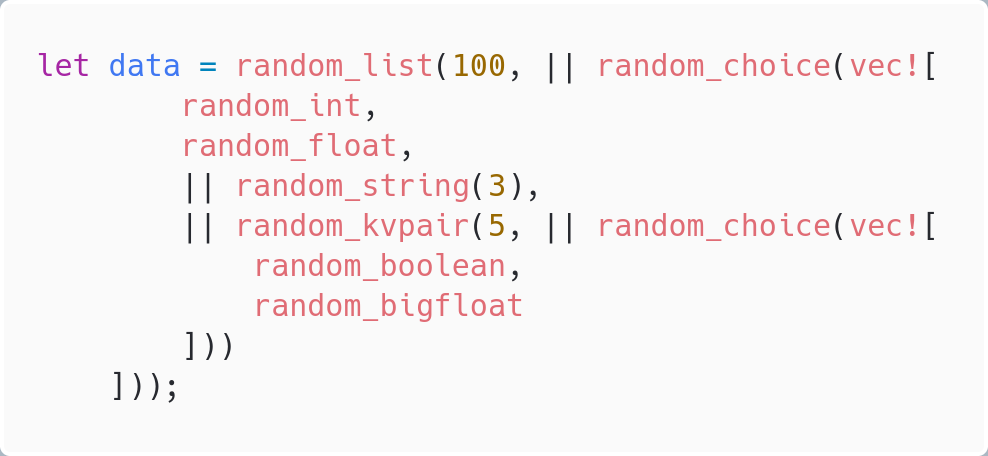
\includegraphics[width=0.5\textwidth]{images/codegen_code.png}
    \caption{Codebeispiel zur Datensatzgenerierung}
    \label{fig:codegen_example}
\end{figure}

\autoref{fig:codegen_example} zeigt den Code, der einen Testdatensatz beschreibt (und generiert). Der Datensatz besteht aus einer Liste mit 100 Elementen, von welchen jedes entweder ein Integer, Float, zufälliger String der Länge 3, oder ein Key-Value-Pair mit Schlüssellänge 5 ist, dessen Wert widerum entweder ein zufälliger Boolean oder Float ist.

Damit möglichst viele Stärken und Schwächen der getesteten Serialisierungsformate abgebildet werden, werden mehrere verschiedene Testdatensätze generiert. Diese variieren in folgenden Metriken:

\begin{itemize}
  \item Nesting-Tiefe
  \item Nesting-Breite
  \item Anzahl Primitive
  \item Homogenität der Primitive
\end{itemize}

\subsection{Python Implementierung}

Die in der Tabelle dargestellten Versionen der verwendeten Softwarekomponenten zeigen, welche spezifischen Tools und Technologien für die Durchführung der Tests genutzt wurden:

\begin{table}[H]
    \centering
    \begin{tabular}{|l|l|}
    \hline
    \textbf{Name} & \textbf{Version} \\ \hline
    Python        & 3.12             \\ \hline
    ijson         & 3.3.0            \\ \hline
    lxml          & 5.3.0            \\ \hline
    msgpack       & 1.1.0            \\ \hline
    protobuf      & 5.28.3           \\ \hline
    \end{tabular}
    \caption{Verwendete Technologien der Messreihe}
\end{table}

\begin{table}[H]
\centering
\begin{tabular}{|l|l|}
\hline
\textbf{Komponente}         & \textbf{Details}                     \\ \hline
Betriebssystem              & Manjaro Linux                        \\ \hline
Prozessor                   & Intel Core i7-13620H                 \\ \hline
Prozessor-Details           & 24 MB Cache, bis zu 4.9 GHz           \\ \hline
Arbeitsspeicher             & 32 GB (2x16 GB DDR5, 4800 MHz)       \\ \hline
\end{tabular}
\caption{Für die Messreihe verwendete Hardware}
\label{tab:hardware}
\end{table}

Die Tests wurden in einem strukturierten und standardisierten Ablauf durchgeführt, wobei spezifische Anpassungen vorgenommen wurden, um die Besonderheiten der getesteten Serialisierungsverfahren zu berücksichtigen. Jeder der generierten Datensätze wurde zunächst geladen und seine Größe im Speicher erfasst, um später als Referenz für die Berechnung der Kompressionsrate zu dienen. Anschließend wurden die Serialisierungs- und Deserialisierungszeiten sowie die resultierende Größe der serialisierten Daten für jede Technologie (JSON, XML, MessagePack und Protocol Buffers) gemessen.

Für XML wurde aufgrund des hohen Speicherverbrauchs bei der Verarbeitung größerer Datensätze ein optimiertes Streamingverfahren eingesetzt. Bei diesem Ansatz wird der Datensatz nicht vollständig im Speicher gehalten, sondern schrittweise verarbeitet. Die XML-Daten werden dabei durch eine rekursive Generierung einzelner XML-Elemente Stück für Stück erzeugt und direkt in eine Datei geschrieben. Dadurch wird der Speicherbedarf unabhängig von der Größe des Datensatzes auf ein Minimum reduziert. Dieses Verfahren ermöglicht es, auch extrem große Datensätze zu serialisieren, ohne den verfügbaren Arbeitsspeicher zu überlasten. Es bildet gleichzeitig typische Anwendungsfälle in realen datenintensiven Szenarien ab, bei denen Ressourcen effizient genutzt werden müssen. Allerdings hat dies solch immense Auswirkungen auf die Serialisierungszeit das für die Bewertung die Ergebnisse von großen Datensätzen mittels XML verworfen wurden.

Protocol Buffers (Protobuf) erhielt ebenfalls spezifische Implementierungen für jede Datensatzart. Diese Maßnahme war notwendig, da eine generische Behandlung in Protobuf zu schlechten Ergebnissen führt, die die tatsächlichen Stärken des Formats nicht widerspiegeln. Mit maßgeschneiderten Protobuf-Definitionen und entsprechenden Serialisierungs- und Deserialisierungsfunktionen konnte eine realistischere Bewertung vorgenommen werden, die den praxisnahen Einsatz des Formats besser abbildet.

Zusätzlich wurde die Hardwareumgebung detailliert protokolliert, um die Ergebnisse im Kontext der zugrunde liegenden Systemressourcen bewerten zu können. Erfasst wurden dabei unter anderem CPU-Modell, Anzahl der logischen Kerne, verfügbare Arbeitsspeicherkapazität und Betriebssystem. Diese Informationen sind wichtig, da sie maßgeblich die Leistung der Serialisierungsverfahren beeinflussen können. Durch die Dokumentation der Hardwarebedingungen wird die Reproduzierbarkeit der Ergebnisse gewährleistet und es können eventuelle Abweichungen bei Tests auf anderen Systemen besser nachvollzogen werden.

Die Tests wurden für jede Kombination aus Datensatz, Technologie und Implementierung über mehrere Wiederholungen durchgeführt, um statistische Schwankungen zu minimieren. Die Ergebnisse, einschließlich aller gemessenen Metriken, wurden in einer strukturierten JSON-Ausgabe gespeichert.

\subsubsection{Probleme und Limitationen}

Ein wesentliches Problem bei den Messungen war die ineffiziente Datenhaltung in Python. Diese führte dazu, dass ein 680 MB großer JSON-Datensatz im Speicher etwa 2 GB beanspruchte, was die Effizienz der Tests erheblich beeinträchtigte.

Die Implementierungen von Protobuf und XML stellten besondere Herausforderungen dar. Insbesondere XML erwies sich aufgrund seines hohen Speicherverbrauchs als problematisch. Bei einigen Datensätzen, wie dem zuvor erwähnten JSON-Datensatz, benötigte die XML-Serialisierung teilweise über 30 GB Arbeitsspeicher. Diese hohen Anforderungen führten dazu, dass XML für besonders speicherintensive Datensätze nicht getestet wurde, da die Tests oft unvorhersehbar fehlschlugen. Selbst wenn die Serialisierung funktionierte, betrugen die Laufzeiten bei der Streaming-Variante für große Datensätze häufig mehr als 10 Minuten, was die Durchführung der Tests unpraktikabel machte.

Es sei jedoch darauf hingewiesen, dass einige dieser Probleme möglicherweise auf die gewählte Implementierung zurückzuführen sind. Python bietet verschiedene XML-Bibliotheken an, die oft auf spezifische Anwendungsfälle optimiert sind. Eine einzige, universelle Implementierung innerhalb des Testskripts, die alle Datensatztypen abdeckt, kann zu Leistungseinbußen führen. Eine detaillierte Untersuchung der unterschiedlichen XML-Bibliotheken und deren Eignung für spezifische Anforderungen wäre hier sinnvoll, würde jedoch den Rahmen dieser Arbeit sprengen.

Protobuf brachte ebenfalls spezifische Schwierigkeiten mit sich. Die ineffiziente Datenhaltung in Python, kombiniert mit dessen vergleichsweise langsamer Programmausführungszeit, machte es notwendig, für jeden Datensatz spezifische Protobuf-Implementierungen zu entwickeln, um eine faire Vergleichsbasis zu schaffen. Die generische Implementierung verursachte aufgrund des hohen Sprach-Overheads erheblichen Ressourcenverbrauch und lange Ausführungszeiten, sodass Protobuf in diesen Fällen sogar von XML in Effizienz und Performance übertroffen wurde.

Ein weiteres Problem betrifft die Limitierungen von Python selbst. Bei JSON-Strukturen mit einer Tiefe von mehr als 100 Ebenen führten die zahlreichen Rekursionsaufrufe dazu, dass Python die Verarbeitung mit einem Fehler abbrach. Dieses Problem ließ sich nicht durch eine Erhöhung der maximalen Rekursionstiefe beheben. Ähnliche Probleme traten auch bei Protobuf auf, das mit Datenstrukturen, die mehr als 50 Ebenen tief waren, nicht korrekt umgehen konnte. In diesen Fällen war die Serialisierung fehlerhaft, und die Deserialisierung konnte nicht erfolgreich abgeschlossen werden.

Einzig und allein MessagePack wies keine bekannten / offensichtlichen Limitationen oder Probleme auf.

Diese Einschränkungen zeigen die praktischen Herausforderungen bei der Verwendung von Python und bestimmten Serialisierungsformaten in ressourcenintensiven Szenarien auf. Sie unterstreichen die Bedeutung einer angepassten Implementierung und realistischen Bewertung der Verfahren unter Berücksichtigung ihrer spezifischen Eigenheiten.

\subsection{Rust}

Die in der Tabelle dargestellten Versionen der verwendeten Softwarekomponenten zeigen, welche spezifischen Tools und Technologien für die Durchführung der Tests genutzt wurden:

\begin{table}[H]
    \centering
    \begin{tabular}{|l|l|}
    \hline
    \textbf{Name} & \textbf{Version} \\ \hline
    Rust          & 1.85             \\ \hline
    serde         & 1.0.215          \\ \hline
    serde\_json   & 1.0.132          \\ \hline
    serde\_xml    & 0.9.1            \\ \hline
    quick\_xml    & 0.37.1           \\ \hline
    protobuf      & 3.7.1            \\ \hline
    \end{tabular}
    \caption{Verwendete Technologien der Messreihe}
\end{table}

\begin{table}[H]
  \centering
  \begin{tabular}{|l|l|}
  \hline
  \textbf{Komponente}         & \textbf{Details}                     \\ \hline
  Betriebssystem              & Manjaro Linux                        \\ \hline
  Prozessor                   & AMD Ryzen 9 5900X                    \\ \hline
  Prozessor-Details           & 64 MB Cache, bis zu 4.9 GHz          \\ \hline
  Arbeitsspeicher             & 32 GB (2x16 GB DDR5, 4800 MHz)       \\ \hline
  \end{tabular}
  \caption{Für die Messreihe verwendete Hardware}
  \label{tab:hardware_rust}
\end{table}

Der Ablauf des Testing-Prozesses geschieht ähnlich zur Python-Implementierung in einem strukturierten und standardisierten Ablauf. Auch hier wird der gesamte Datensatz zunächst in den Speicher geladen, um IO-Performanz von der Messung auszuschließen. Ebenso werden alle Datensätze sequentiell geladen und mehrfach für jedes Serialisierungsformat serialisiert und anschließend deserialisiert, um statistische Schwankungen zu minimieren. Zur Ausgabe der Ergebnisse wird das gleiche, JSON-basierte Format verwendet. Dadurch können die Messergebnisse mit den gleichen Tools verarbeitet und analysiert werden. Ebenso wurden die gleichen Daten über die Hardwareumgebung erfasst, wie es für die Python-Implementierung der Fall ist.

Die Implementierung geschieht mit Hilfe des weit-verbreiteten \cite{serde} Frameworks ``Serde''. Alle getesteten Formate außer Protobuf werden von Serde unterstützt. (Protobuf unterstützt aktuell nur Deserialisierung, aber keine Serialisierung. Deshalb wird auf das zusätzliche Crate ``protobuf'' zurückgegriffen.). Dazu wird zunächst eine generische Implementierung der beiden Traits ``Serialize'' und ``Deserialize'' umgesetzt. Innerhalb dieser Implementierung wird beschrieben, wie Serde den zentralen Datentyp in Serde-Datentypen transformieren soll. Anschließend können vorgegebene Funktionen genutzt werden, um die Serialisierung und Deserialisierung in verschiedene Formate vorzunehmen. Die Implementierung fällt daher vergleichsweise kompakt und simpel aus. Für Protobuf werden zunächst über den Protobuf Compiler (protoc) eine .proto-Datei generiert. Mit Hilfe dieser Datei und des Rust-Crates ``protobuf'' kann über einen einzigen Funktionsaufruf die Serialisierung und Deserialisierung implementiert werden. Anders als bei Python zeigt die automatisch generierte Protobuf-Datei im Test gute Performanz bei der Serialisierung.

\subsubsection{Probleme und Limitationen}

Ausschließlich XML führte zu Problemen in der Implementierung. Das mit Serde mitgelieferte ``serde\_xml'' formatierte bei der Serialisierung die primitiven Datenwerte ohne Delimitation oder Tags. Der resultierende Datensatz war gänzlich unbrauchbar. Zur Behebung wurde das externe Crate ``quick-xml'' verwendet. Dieses verwendet die gleichen Traits, die auch Serde verwendet. Somit entfällt eine separate Implementierung von XML. Leider zeigt auch diese Implementierung Probleme in Bezug auf den Speicherverbrauch. Bei den größeren Datensätzen sind 32 GB Arbeitsspeicher teilweise nicht ausreichend, um den gesamten Datensatz zu serialisieren/deserialisieren.

\section{Ergebnisauswertung}

Im folgenden werden die entstandenen Ergebnisse der Implementationen gegenübergestellt und nach den zuvor genannten Metriken bewertet.

\subsection{Serialisierungs- \& Deserialisierungszeit}

Die Messergebnisse variieren je nach Aufbau des Datensatzes. 

\begin{figure}[h]
  \centering
  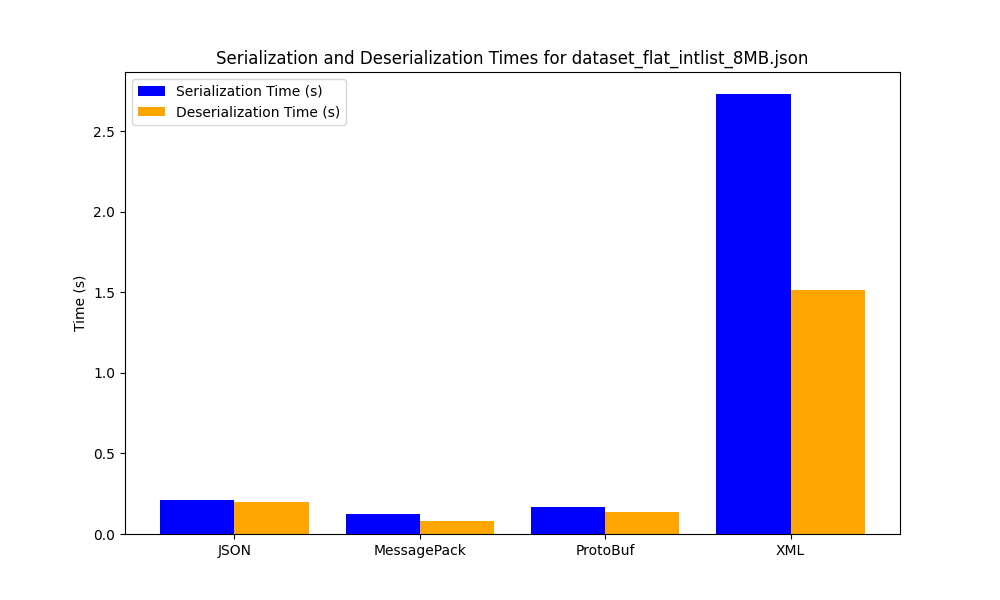
\includegraphics[width=0.5\textwidth]{images/graphs/python_dataset_flat_intlist_8MB_json_combined_times.png}
  \caption{Serialisierungs- und Deserialisierungszeit 8MB Integerliste in Python}
  \label{fig:python_serde_8mb_intlist}
\end{figure}

\begin{figure}[h]
  \centering
  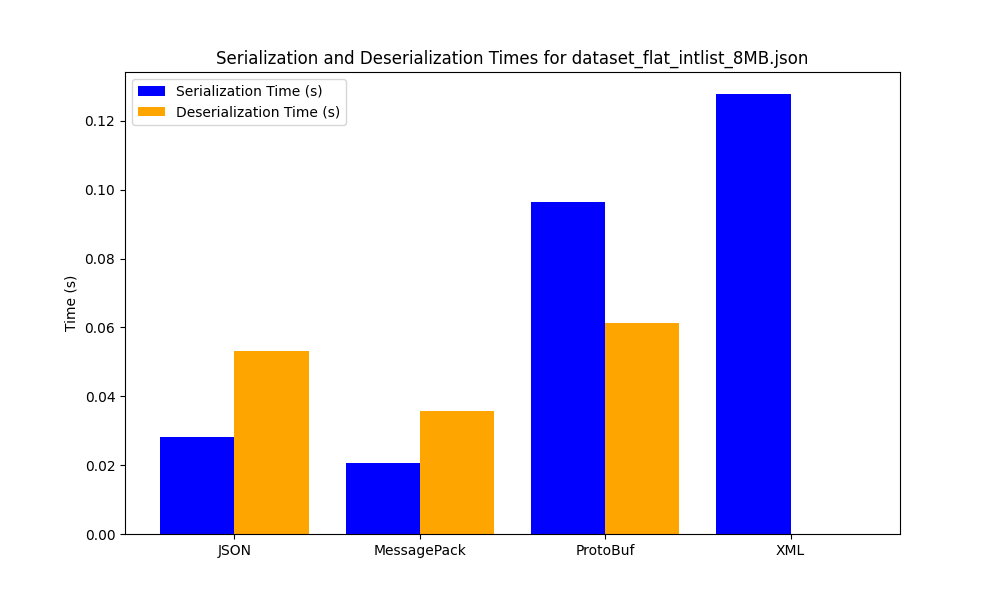
\includegraphics[width=0.5\textwidth]{images/graphs/rust_dataset_flat_intlist_8MB_json_combined_times.png}
  \caption{Serialisierungs- und Deserialisierungszeit 8MB Integerliste in Rust}
  \label{fig:rust_serde_8mb_intlist}
\end{figure}

\newpage

\autoref{fig:python_serde_8mb_intlist} und \autoref{fig:rust_serde_8mb_intlist} zeigen die Serialisierungs- und Deserialisierungslaufzeiten der getesteten Formate für eine flache Liste von 32-Bit Integern von jeweils ca. 8MB. Zu sehen ist die allgemein um ca. eine Größenordnung kürzere Laufzeit aller Formate in Rust gegenüber Python, was dadurch begründet werden kann, dass Python eine interpretierte Programmiersprache ist. Mit Ausnahme von XML schneiden in der Python-Implementierung alle Formate ähnlich gut ab. In der Rust-Implementierung sticht zusätzlich Protobuf als langsameres Format hervor. Dies wird dadurch begründet, dass die Python-Implementierung eine optimierte Version des Protobuf-Schemas für die Datenstrukturen verwendet. 

XML sticht in beiden Implementierungen als langsamstes Format hervor. Die Deserialisierung von XML-Datensätzen schlägt in der Rust-Implementierung auch bereits bei kleinen Datensätzen ($\ge$ 4MB) fehl. In Python ist die Serialisierung von XML ca. 7 mal langsamer als das ansonsten langsamste Format, in Rust immerhin nur um den Faktor 1.3 im Vergleich zu Protobuf, und ebenfalls um den Faktor 7 zum ansonsten langsamsten Format. Diese Messergebnisse bestätigen die von \textit{Hericko et al.}. In deren Resultaten erfassen diese eine Spanne von 5-9 \cite[ Kapitel 5]{10.1145/944579.944589} zwischen den binären und nichtbinären Formaten. Diese relativ langsame Serialisierungs- und Deserialisierungszeit wird dadurch begründet, dass XML arbiträre Metadaten mit Tags assoziieren kann und die Datenhaltung und das Parsing damit erheblich komplexer ist als bei anderen Formaten ohne diese Funktionen \cite[Kapitel 4.1]{10.1145/944579.944589}.

\begin{figure}[h]
  \centering
  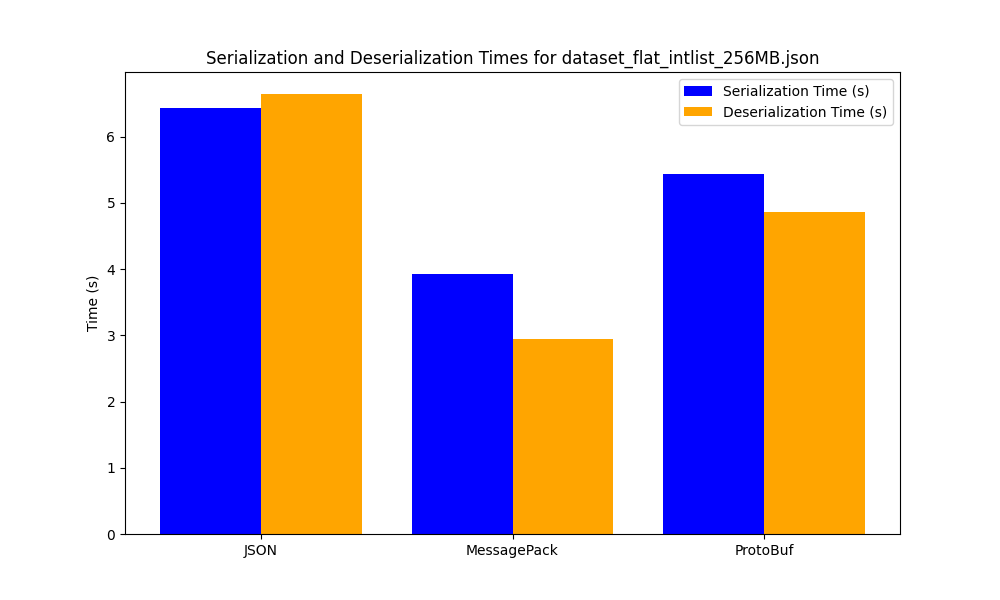
\includegraphics[width=0.5\textwidth]{images/graphs/python_dataset_flat_intlist_256MB_json_combined_times.png}
  \caption{Serialisierungs- und Deserialisierungszeit 256MB Integerliste in Python}
  \label{fig:python_serde_256mb_intlist}
\end{figure}

\begin{figure}[h]
  \centering
  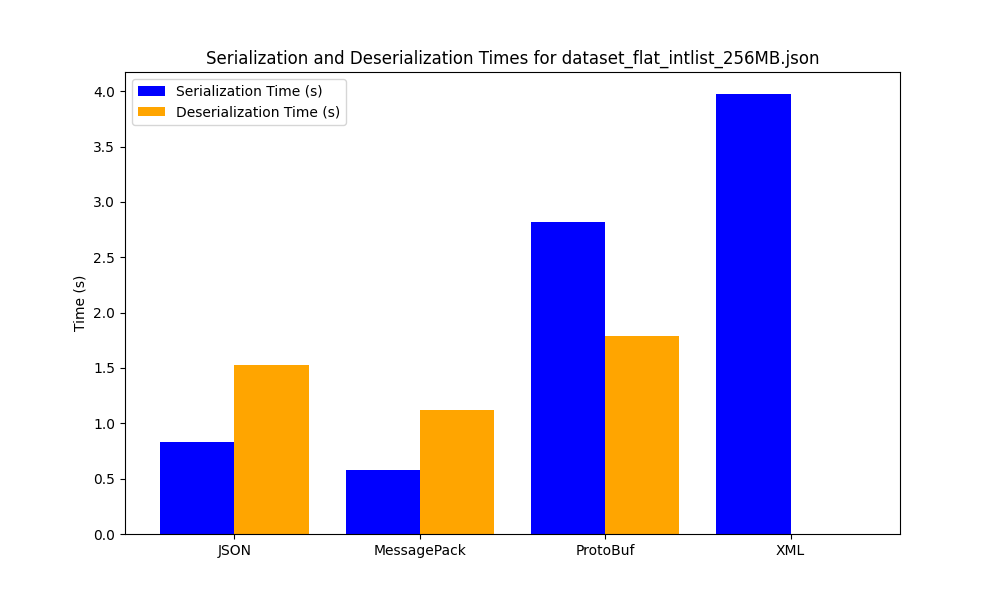
\includegraphics[width=0.5\textwidth]{images/graphs/rust_dataset_flat_intlist_256MB_json_combined_times.png}
  \caption{Serialisierungs- und Deserialisierungszeit 256MB Integerliste in Rust}
  \label{fig:rust_serde_256mb_intlist}
\end{figure}

\autoref{fig:rust_serde_256mb_intlist} und \autoref{fig:python_serde_256mb_intlist} zeigen die Serialisierungs- und Deserialisierungslaufzeiten von ähnlichen, aber größeren Datensätzen mit jeweils 256MB an Nutzdaten. Während die absoluten Laufzeiten größer ausfallen, sind die relativen Laufzeiten der Formate untereinander nahezu identisch. Dies deutet darauf hin, dass alle getesteten Implementierungen annähernd linear skalieren. Auch diese Beobachtung bestätigt die Ergebnisse von \textit{Hericko et al.} \cite[Figure 9]{10.1145/944579.944589}.

\begin{figure}[h]
  \centering
  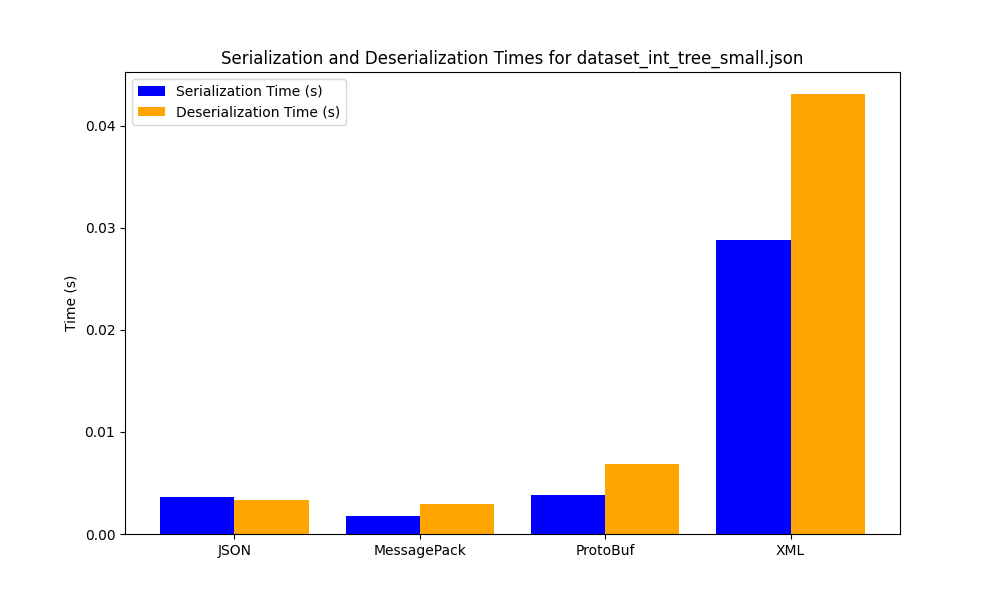
\includegraphics[width=0.5\textwidth]{images/graphs/python_dataset_int_tree_small_json_combined_times.png}
  \caption{Serialisierungs- und Deserialisierungszeit Integerbaum in Python}
  \label{fig:python_serde_8mb_inttree}
\end{figure}

\begin{figure}[h]
  \centering
  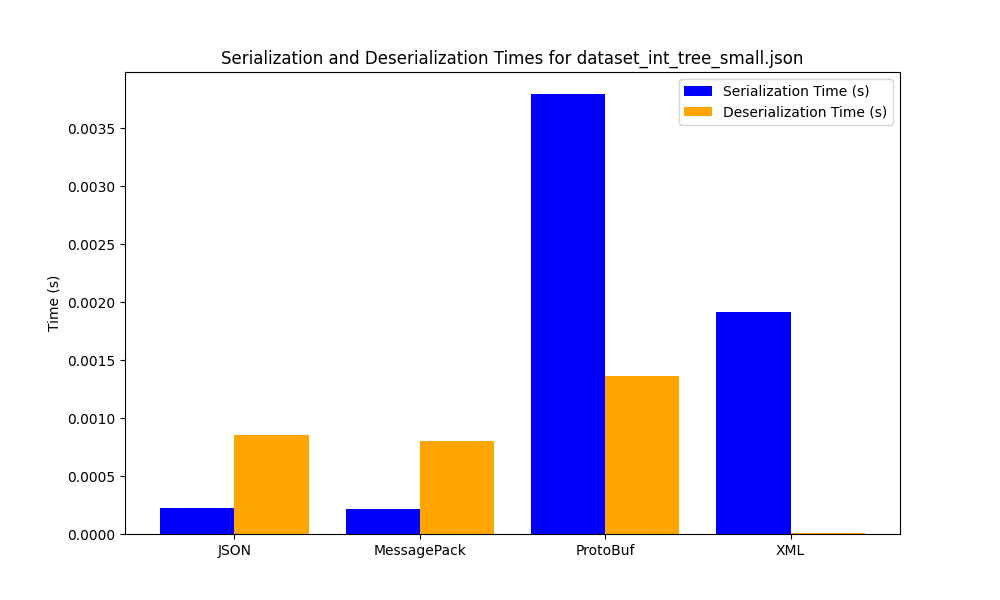
\includegraphics[width=0.5\textwidth]{images/graphs/rust_dataset_int_tree_small_json_combined_times.png}
  \caption{Serialisierungs- und Deserialisierungszeit Integerbaum in Rust}
  \label{fig:rust_serde_8mb_inttree}
\end{figure}

\autoref{fig:rust_serde_8mb_inttree} und \autoref{fig:python_serde_8mb_inttree} zeigen die Laufzeiten für eine Baumstruktur, die aus 4 Ebenen an Knoten besteht. Jeder Knoten speichert einen 32-Bit Integer, sowie 8 Kind-Knoten. Die Python-Implementierung zeigt ähnliche Performanz im Vergleich zu flachen Listen. Die relative Performanz der Formate in der Rust-Implementierung ist ebenfalls nahezu identisch, jedoch sticht Protobuf hier durch eine massiv erhöhte Serialisierungs- und Deserialisierungszeit hervor. Dies deutet darauf hin, dass komplexe Datenstrukturen in Protobuf vergleichsweise ineffizient serialisiert werden.

\newpage

\subsection{Kompressionsrate}

Die Kompressionsrate errechnet sich wie folgt:

$$ K = \frac{Bytes_\text{roh}}{Bytes_\text{serialisiert}} $$

Dabei kann $ Bytes_\text{roh} $ entweder die tatsächliche Größe der Datenobjekte im Arbeitsspeicher sein, oder die Größe der Nutzlast. \autoref{fig:compression_ratios} zeigt die Kompressionsraten von Ersterem, wobei sich die Größe der Datenobjekte auf die Python-Implementierung bezieht. Werden nur die Nutzdaten bewertet, wird die gesamte Ergebnisreihe um einen konstanten Faktor skaliert. Für den Vergleich mehrerer Implementierungen ist dieser Faktor unerheblich, da nur die relativen Messungen innerhalb einer Implementierung relevante Vergleichsmetriken bilden.

\begin{figure*}[t] % Sternchen sorgt dafür, dass die Grafik über beide Spalten geht
  \centering
  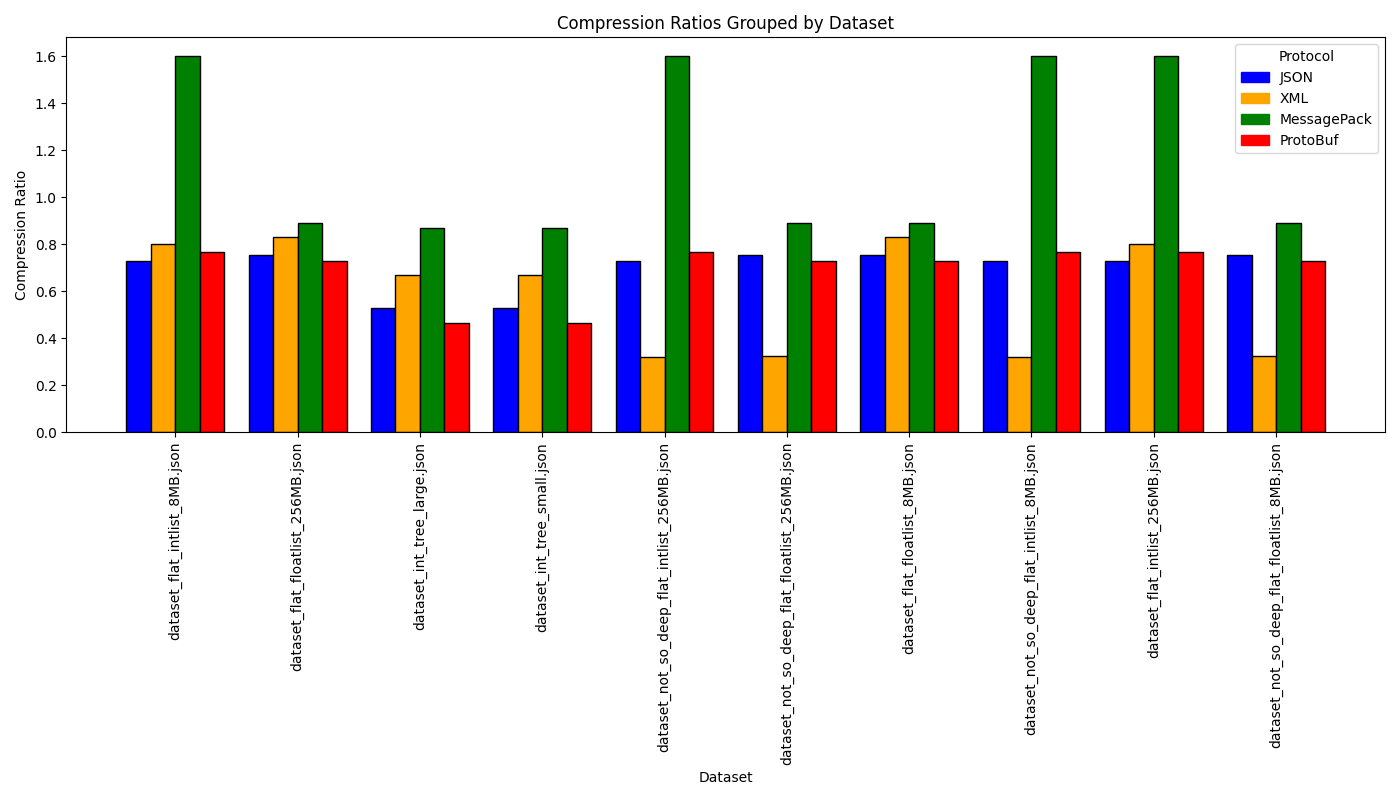
\includegraphics[width=\textwidth]{images/graphs/combined_compression_ratios.png} % Breite über gesamte Seitenbreite
  \caption{Relative Kompressionsraten von Python Objekten}
  \label{fig:compression_ratios}
\end{figure*}

Die Grafik zeigt, dass erneut XML als das mit Abstand suboptimalste Format herraussticht. Da jeder Datenpunkt mit einem eigenen Paar aus Delimitierungs-Tags gekennzeichnet sein muss, ist das Verhältnis von Nutzlast zu Metainformationen deutlich geringer als in allen anderen Formaten. Es ergibt sich eine durchschnittliche Kompressionsrate von $\approx 0.04$ über alle getesteten Datensätze. Das bedeutet, dass jedes Byte eines Python-Objektes ca. 25 Bytes an serialisierten Daten produziert. Diese Kompressionsrate verschlechtert sich mit zunehmender Tiefe und Komplexität der Datenstrukturen.

Alle anderen Formate erreichen durchgehend Kompressionsraten $\geq 1$, was bedeutet, dass die serialisierte Datenmenge kleiner ist als die Python-Datenobjekte. Simple Datenstrukturen wie Listen werden von Protobuf und Messagepack am effizientesten serialisiert, wobei Messagepack Integer und Protobuf Floats effizienter kodiert. Auffällig ist zudem die extrem hohe Kompressionsrate des Integer-Baum-Datensatzes, bei dem Protobuf einen Wert von $61.74$ erreicht. Daraus wird klar, dass die Metadaten, die Python für das Speichern von solchen Strukturen benötigt, sehr platzsparend von Protobuf (und auch den anderen Formaten) serialisiert werden können.

JSON bildet ein durchweg gutes Mittelmaß über alle Datensätze. Die durchschnittliche Kompressionsrate von $\approx 4.2$ zeigt, dass auch nichtbinäre Formate gegenüber der nativen Repräsentation von Python-Objekten effizient serialisiert werden können.

\subsection{Implementierungsgüte}
Im folgenden wurden alle Messeregebnisse normalisiert und ein Durschnitt erfasst um die zwei Sprachen untereinander vergleichen zu können. Werte die größer Eins sind bedeuten das Rust hier um diesen Faktor besser performt hat.

\begin{table}[H]
    \resizebox{\columnwidth}{!}{% Adjust to fit column width
    \begin{tabular}{|l|l|l|l|l}
    \cline{1-4}
    \textbf{Format} & \textbf{Serialisierung} & \textbf{Deserialisierung} & \textbf{Kompression} &  \\ \cline{1-4}
    JSON               & 7.858018                & 4.026984                  & 0.224557               &  \\ \cline{1-4}
    MessagePack        & 5.909328                & 2.354893                  & 0.205478               &  \\ \cline{1-4}
    ProtoBuf           & 1.665640                & 1.915003                  & 0.106578               &  \\ \cline{1-4}
    XML                & 10.588883               & -                         & 86.795813              &  \\ \cline{1-4}
    \end{tabular}}
    \caption{Relative Performance von Rust gegenüber Python}
\end{table}

\newpage

Python zeigt in der Kompression durchweg bessere Ergebnisse als Rust. Dies liegt daran, dass Python-Objekte im Speicher eine vergleichsweise große Größe aufweisen, was dazu führt, dass die Daten nach der Serialisierung stärker komprimiert erscheinen. In der Serialisierungs- und Deserialisierungsgeschwindigkeit hingegen übertrifft Rust Python deutlich. Dies ist auf die native Kompilierung von Rust und die damit verbundene Optimierung auf niedriger Ebene zurückzuführen, wodurch Serialisierungsbibliotheken effizienter arbeiten können. Die Ergebnisse verdeutlichen, dass Rust besonders in Szenarien mit hohen Anforderungen an die Verarbeitungsgeschwindigkeit Vorteile bietet, während Python durch seine Speicherrepräsentation eine effektivere Kompression erreicht.

Wenn man auf die einzelnen Serialisierungsformate schaut, sieht man allerdings, dass gerade die binären Formate nicht so stark profitieren von der Sprachimplementierung wie die nicht-binären JSON und XML.

\subsection{Ressourcenverbrauch}
Die Ergebnisse zeigen, dass XML im Vergleich der getesteten Formate den höchsten Ressourcenverbrauch aufweist. Insbesondere bei großen Objekten ist der Speicherbedarf exorbitant: Ein 2-GB-Objekt führte zu einem Speicherverbrauch von über 32 GB in der verwendeten Implementierung, sowohl in Python als auch in Rust. Dies macht XML für speicherintensive Anwendungen unpraktisch, insbesondere in ressourcenbeschränkten Umgebungen wie Embedded-Systemen oder IoT-Geräten. JSON zeigte sich als moderat und benötigte etwa den gleichen Speicherplatz des originalen Objekts, was auf die Textstruktur des Formats zurückzuführen ist. MessagePack erwies sich als das ressourcenschonendste Format: Es war nicht nur das schnellste, sondern erzeugte auch keine signifikanten Ausschläge im Ressourcenmonitor. Damit eignet es sich hervorragend für Systeme, bei denen geringe Latenz und niedriger Speicherverbrauch essenziell sind, beispielsweise in Echtzeitanwendungen oder mobilen Geräten. Protobuf zeigte einen ähnlichen Ressourcenverbrauch wie JSON, mit einer tendenziell geringeren Speicherbelastung. Es bietet damit eine gute Balance zwischen Effizienz und Flexibilität, insbesondere in leistungsorientierten Anwendungen wie der Kommunikation zwischen Microservices.

\subsection{Nutzbarkeit / Wartbarkeit}
In Bezug auf Nutzbarkeit und Wartbarkeit erwiesen sich MessagePack und JSON als die angenehmsten Formate. Beide ermöglichen eine dynamische Serialisierung und Deserialisierung von Objekten ohne zusätzliche Konfigurationsschritte, was die Entwicklung deutlich vereinfacht. JSON bietet dabei den zusätzlichen Vorteil, dass es in nahezu allen gängigen Programmiersprachen nativ unterstützt wird, wodurch Daten direkt inspiziert und debuggt werden können. MessagePack glänzt durch seine Effizienz und Einfachheit, allerdings führt die Community-Driven-Entwicklung dazu, dass für manche Programmiersprachen mehrere Implementierungen existieren. Diese können sich in ihrer Entwicklungsgeschwindigkeit und Funktionsweise unterscheiden, was langfristig potenzielle Kompatibilitätsprobleme oder Mehraufwand bei der Auswahl einer geeigneten Implementierung bedeuten könnte.

\newpage

XML und Protobuf hingegen erfordern einen größeren Implementierungsaufwand. Bei XML müssen Serialisierungs- und Deserialisierungsfunktionen implementiert werden, wobei verschiedene Bibliotheken zur Verfügung stehen, die unterschiedliche Funktionalitäten und Erweiterungen bieten. Diese Fragmentierung kann in der Entwicklung zusätzliche Entscheidungen und Abwägungen erfordern. Protobuf arbeitet mit einer vorab definierten .proto-Datei, die eine klare Struktur vorgibt und die langfristige Wartbarkeit in großen Projekten verbessert. Diese Standardisierung vermeidet inkompatible Implementierungen zwischen verschiedenen Sprachen, bietet jedoch weniger Flexibilität im Vergleich zu JSON oder MessagePack. Zudem erfordert die Arbeit mit Protobuf Erfahrung im Umgang mit Schema-Design, um eine optimale Datenstruktur zu gewährleisten. Python stößt bei der Arbeit mit tief verschachtelten Strukturen an Grenzen, was den Implementierungsaufwand für generische Lösungen zusätzlich erhöht.

\textbf{Langfristige Überlegungen:}
Die langfristige Nutzbarkeit und Wartbarkeit hängen stark von der Entwicklung und Unterstützung der jeweiligen Implementierungen ab. JSON und Protobuf profitieren von ihrer langjährigen Etablierung und der breiten Unterstützung durch offizielle und gut dokumentierte Bibliotheken. MessagePack hingegen, trotz seiner Effizienz, birgt Risiken durch die Vielzahl an Community-Implementierungen, die sich unterschiedlich schnell und unabhängig voneinander weiterentwickeln können. XML, obwohl etabliert, wird durch seine vergleichsweise komplexe Handhabung und die eingeschränkte Performance zunehmend weniger attraktiv für moderne Entwicklungsprojekte.

Insgesamt sind JSON und Protobuf aufgrund ihrer Standardisierung und umfassenden Unterstützung die besseren Optionen für langfristige Projekte, während MessagePack für kleinere, performancekritische Anwendungen optimal ist. XML bleibt eine Wahl für spezialisierte Anwendungsbereiche, bei denen strukturierte Validierung im Vordergrund steht.


\section{Fazit}

Im Folgenden wird eine Schlussfolgerung aus den Messergebnissen und bisherigen Resultaten abgeleitet.

\subsection{JSON}
JSON bewährte sich in den Tests als vielseitiges und einfach zu nutzendes Format. Durch seine menschenlesbare Struktur und die breite Unterstützung in nahezu allen gängigen Programmiersprachen eignet es sich besonders für Web-APIs, Konfigurationsdateien und Anwendungen, bei denen die Lesbarkeit eine zentrale Rolle spielt. Allerdings zeigte sich JSON wie erwartet in der Kompression und Performance den binären Formaten unterlegen, was insbesondere bei großen Datensätzen deutlich wurde. Die Ergebnisse stimmen mit bisherigen Studien überein, die JSONs Effizienz für die meisten allgemeinen Anwendungen bestätigen, jedoch auf Schwächen bei speicherintensiven Szenarien hinweisen. Trotz seiner Nachteile bleibt JSON eine ausgezeichnete Wahl für Szenarien, die eine Balance zwischen Lesbarkeit und Funktionalität erfordern.

\subsection{MessagePack}
MessagePack überzeugte in den Tests durch seine herausragende Performance und die exzellente Speicherkompression. Es zeigte sich als das ressourcenschonendste Format, mit kurzen Serialisierungszeiten und minimalem Speicherbedarf. Besonders in ressourcenbeschränkten Umgebungen wie IoT- oder Echtzeitsystemen glänzt MessagePack. Ähnliche Erkenntnisse finden sich auch in den Analysen von ProgrammerAL \cite{ProgrammerAL_SerializationBenchmarks}, wo MessagePack im Vergleich zu anderen Formaten wie Protobuf und JSON hinsichtlich Geschwindigkeit und Speicherverbrauch überlegen war. Für Szenarien, in denen Effizienz entscheidend ist, stellt es eine ausgezeichnete Wahl dar.

\subsection{ProtoBuf}
Protobuf zeigte in den Tests gute Ergebnisse bei der Kompression und Serialisierungszeit, insbesondere bei einfacheren Datensätzen. Für komplexe Strukturen nahm die Laufzeit jedoch spürbar zu, was die Effizienz im Vergleich zu MessagePack etwas beeinträchtigte. Seine strikte Typisierung und die Nutzung von Schema-Dateien (.proto) machen Protobuf besonders für stark typisierte Anwendungen attraktiv, wie sie in Microservices-Architekturen häufig vorkommen. Diese Ergebnisse decken sich mit der Studie von Nate \cite{Nate10_2024}, die Protobuf für Websockets hinsichtlich Effizienz und Strukturierung als eine der besten Optionen bewertet hat. Protobuf bleibt eine ausgezeichnete Wahl für Systeme, die auf klar definierte Strukturen und effiziente Datenübertragung angewiesen sind.

\subsection{XML}
XML ist ein langsames und schwierig aufzusetzendes Format. Als es erschaffen wurde hat es einige Probleme gelöst doch über die Jahre wurden für viele Probleme spezialisierte Lösungen geschaffen die deutlich effizienter sind als XML. Auch in den hier durchgeführten Testreihen hat sich die allgemeine Komplexität als auch ein sehr hoher Ressourcenverbrauch deutlich gezeigt \cite{Pommerenig_2019}. XML wird meist noch noch für Legacy Projekte verwendet doch in Bereichen der Datenübertragung oder in modernen Webanwendungen haben andere Serialisierungsformate meist die Oberhand.


\section{Ausblick}

In Zukunft wäre es möglich diese Metriken zu erweitern sowie weitere Formate hinzuzufügen als auch die selbe Umgebung in mehreren Programmiersprachen zu testen um etwaige Implementierungsunterschiede durch eine größere Menge an Daten auszumerzen. Auch eine Aufteilung in die einzelnen Schritte eines Serialisierungs/Deserialisierungsprozess könnte interessante Erkenntnisse über etwaige Bottlenecks aufzeigen die sich in den Sprachen ergeben wie es in der bisher öfters genannten Arbeit zu den Vergleichen zwischen Java und .NET gemacht wurde \cite{10.1145/944579.944589}. 

Ein weiteres interessantes Format für zukünftige Untersuchungen könnte Bebop sein, ein binäres Serialisierungsformat von Betwixt Labs. Bebop wurde speziell für Hochleistungsanwendungen entwickelt und verspricht minimalen Overhead bei gleichzeitig hoher Effizienz. Da dieses Format erst nach Abschluss der Arbeit entdeckt wurde, konnte es nicht in die Tests einbezogen werden. Eine zukünftige Analyse könnte jedoch spannende Einblicke in seine Leistung im Vergleich zu anderen Formaten wie Protobuf und MessagePack liefern. \cite{bebop_serialization}

% Bibliographie entweder direkt hier eingeben (nur im Notfall)...
%\begin{thebibliography}{9}
%\bibitem{ACM2019}
%ACM.
%\newblock How to classify works using ACM's computing classification system.
%\newblock \url{http://www.acm.org/class/how_to_use.html}.
%
%\bibitem{Ivory2001}
%M.~Y. Ivory and M.~A. Hearst.
%\newblock The state of the art in automating usability evaluation of user
%  interfaces.
%\newblock {\em ACM Comput. Surv.}, 33(4):470--516, 2001.
%
%\end{thebibliography}

% ... oder die Bibliographie mit Hilfe von BibTeX generieren,
% dies ist auf jeden Fall die bessere Lösung und sollte nach
% Möglichkeit immer verwendet werden:
\newpage
\bibliographystyle{abbrv}
\bibliography{literatur} % Daten aus der Datei literatur.bib verwenden.

\end{document}
